% id: 67-h6
% book: 개념원리 중학 3-1 · 06 곱셈 공식
% section: 핵심문제 익히기
% figure: crop:fig-67-h6.png
% answer: $40x^2+7x-3$
% answer_source: 본문 답
% variant_level: 0 (원본 전사)
% 이 파일은 build.mjs 가 items.json 에서 만든다. 고칠 때는 items.json 을 고친다.
\smash{\raisebox{1.5mm}{\dmkichul{개념원리 중학 3-1 67쪽 핵심문제 6}}}
\noindent\begin{minipage}[t]{0.58\linewidth}\vspace{0pt}\raggedright 오른쪽 그림과 같이 가로, 세로의 길이가 각각 $8x$, $5x$인 직사각형에서 가로의 길이는 $3$만큼 늘이고 세로의 길이는 $1$만큼 줄여서 만든 직사각형의 넓이를 구하시오.\end{minipage}\hfill\begin{minipage}[t]{0.4\linewidth}\vspace{0pt}\centering \setlength{\dmfigw}{101.9pt}\ifdim\dmfigw>\linewidth\setlength{\dmfigw}{\linewidth}\fi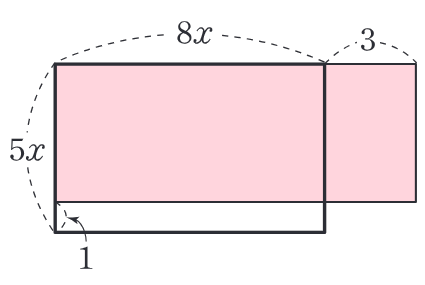
\includegraphics[width=\dmfigw]{figures/fig-67-h6.png}\end{minipage}\par
